\begin{ex}
(Ufla) O movimento de uma partícula é definido pela lei: “Em cada unidade de tempo, a partícula sempre se movimenta de uma unidade de espaço para a direita ou para a esquerda, com igual probabilidade”
No instante inicial, a partícula se encontra na posição 0. Qual a probabilidade, após 5 unidades de tempo, da partícula se encontrar na posição 2?

\begin{center}
    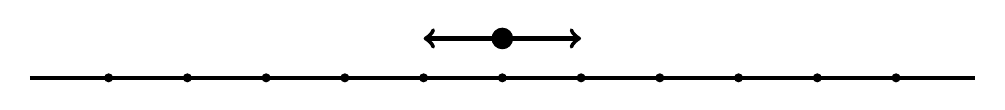
\begin{tikzpicture}
     \draw [ultra thick] (0,0)--(12,0);\draw (1,0) [fill] circle [radius = .05];\draw (2,0) [fill] circle [radius = .05];\draw (3,0) [fill] circle [radius = .05];\draw (4,0) [fill] circle [radius = .05];\draw (5,0) [fill] circle [radius = .05];\draw (6,0) [fill] circle [radius = .05];\draw (7,0) [fill] circle [radius = .05];\draw (8,0) [fill] circle [radius = .05];\draw (9,0) [fill] circle [radius = .05];\draw (10,0) [fill] circle [radius = .05];\draw (11,0) [fill] circle [radius = .05];\draw (6,.5) [fill] circle [radius = .13];
     \draw [ultra thick] [->] (6,.5)--(7,.5); \draw [ultra thick] [<-]  (5,.5)--(6,.5);
    \end{tikzpicture}
\end{center}
   \begin{enumerate}[(a)]
   \item 1
   \item $\frac{1}{2^5}$
   \item 0
   \item $\frac{1}{2}$
   \end{enumerate}
     \begin{sol}
        resposta: c\\
        não dá para estar na posição 2 em 5 unidades de tempo  \hspace{0,3cm}$ \therefore \hspace{0,2cm} p=0$
     \end{sol}
\end{ex}